\documentclass[UTF8]{ctexart}
\usepackage{fancyhdr}
\usepackage{geometry}
\usepackage{fontspec}
\usepackage{tocloft}
\usepackage{hyperref}
\usepackage[normalem]{ulem}
\usepackage{color}
\usepackage{enumitem}
\usepackage{tcolorbox}
\usepackage{graphics}

\geometry{a4paper, margin=1in}

\pagestyle{fancy}
\fancyhf{}
\fancyhead[R]{nim移植LoongArch}
\fancyfoot[C]{\thepage}

\author{赵禹惟}
\date{2024.12.25}

% 规范url颜色
\hypersetup{
	colorlinks=true,
	linkcolor=black,
	urlcolor=[RGB]{0, 102, 204},
	filecolor=[RGB]{0, 102, 204}
}

% 一些引用
\def\nimGitRepo{https://github.com/nim-lang/Nim}
\def\nimPR#1{\nimGitRepo/pull/#1}
\def\nimIssue#1{\nimGitRepo/issues/#1}

% 目录题头
\renewcommand{\cftsecleader}{\cftdotfill{\cftdotsep}}
\renewcommand{\contentsname}{\begin{center}\fontsize{24}{30}\selectfont \heiti 目\hspace{1em}录\end{center}}

% 规范subsection和subsubsection格式
\ctexset{
	subsection={
		format=\raggedright\textbf,
		name={},
		number=\arabic{section}.\arabic{subsection},
		beforeskip=0em,
		afterskip=0em,
	},
	subsubsection={
		format=\raggedright\hspace{2em}\textbf,
		name={},
		number=\arabic{section}.\arabic{subsection}.\arabic{subsubsection},
		beforeskip=0em,
		afterskip=0em,
	}
}

\begin{document}

% 封面设计
\begin{titlepage}
    \begin{center}
    	\vspace*{4cm}
        \line(1,0){450} \\ 
        [5mm]
        {\fontfamily{SimSun}\fontsize{36}{25}\selectfont \textbf{基于开源系统开发应用程序}} \\
        \line(1,0){450} \\
        \hspace{35mm}
        \begin{flushright}
        		{\fontfamily{Times New Roman}\fontsize{25}{25}\selectfont {-- nim移植LoongArch}} \\
		\end{flushright}
    \end{center}
    
    \vspace{80mm}\hspace{-35mm}
    
    \begin{flushright}
    		{\fontfamily{SimSun}\fontsize{20}{25}\selectfont {
			\textbf{队伍名称:}nimble \\
             \textbf{成员:}蔺春名,赵禹惟,李佳潼 \\
             \textbf{创建日期:}2024.12.06 \\}}
    \end{flushright}
\end{titlepage}

% 目录设计
\tableofcontents
\newpage

% 项目背景与目标
\section{项目背景与目标} %1
	\subsection{项目背景} %1.1
	Nim是一个静态系统编程语言,LoongArch是龙芯中科基于CPU研制和生态建设积累推出的自主指令系统架构。在先前的研究中,Nim已经基本实现了在LoongArch上的迁移,其GitHub上的开源项目仓库如下: \\
	\hspace*{2em}\textcolor[RGB]{0, 102, 204}{\underline{\url{https://github.com/nim-lang/Nim.git}}}  \\
	\hspace*{2em}我们的工作是基于已有的迁移上进行的。Nim项目已有的迁移成果如下:
	\begin{enumerate}[leftmargin=3.5em]
		\item 在$ install.ini $增添支持:\underline{\url{\nimPR{23672}}}
		\item 为Nim的符号常量hostCPU增添可能的项 "loongarch64", etc.  \\\underline{\url{\nimPR{19233}}}
	\end{enumerate}
	\hspace*{2em}但是,目前缺少对LoongArch架构的完美支持: \\
	\hspace*{2em}我们尝试在LoongArch架构主机上使用Nim时发现,不但无法按照官方索引安装Nim编译器,而且即使通过源码编译安装也仍然失败。 \\
	\hspace*{2em}具体详情我们小队已经报告到Nim的官方仓库上,详见: \\
	\hspace*{2em}\underline{\url{\nimIssue{24118}}} \\
	\hspace*{2em}另一方面,在后续安装成功后,我们运行了Nim的官方测试用例,发现在LoongArch架构上的一些测试用例没有正常通过。
	\subsection{项目目标} %1.2
	正如上述,在Nim的官方仓库中,LoongArch的迁移工作已经有一定的进展,但是仍存在一些问题需要解决。
	\begin{itemize}[leftmargin=3.5em]
		\item 添加对LoongArch的安装支持
		\item 完善对LoongArch的运行支持(通过测试用例)
	\end{itemize}
	\hspace*{2em}通过如下链接可以访问我们在现有的迁移成果基础上的进一步开发:\\
	\hspace*{2em}\textcolor[RGB]{0, 102, 204}{\underline{\url{https://gitlab.eduxiji.net/T202410423994345/project2608128-274097.git}}} \\
	\hspace*{2em}这是由git管理的2024年全国大学生操作系统竞赛的龙芯相关项目 --- “基于开源操作系统开发应用程序-nim移植LoongArch”。

% 开发环境准备
\section{开发环境准备} %2
	\subsection{前情引入} %2.1
	在将Nim编译器移植到LoongArch架构的过程中,我们需要配置一个完整的开发环境,确保工具链和编译器能够支持RISC64le架构。LoongArch处理器架构是龙芯系列处理器的核心架构,具有RISC(简化指令集计算机)的特性,并且基于RISC64le架构实现,即采用64位架构且字节序为小端排序。RISC64le时RISC-V架构的一个变种,借鉴了RISC-V的一些理念,并加入了本地的指令集扩展。
	\subsection{必要工具和依赖} %2.2
	Nim编译器在进行跨平台移植时,通常会通过本机编译生成目标平台的C代码,再通过C编译器进行编译,最终生成可执行文件(.exe)。为了确保开发工作顺利进行,需要安装以下工具和依赖项:
	\begin{itemize}[leftmargin=3.5em]
		\item Nim及其csource源码: 用于编译Nim编译器 \\
				{\underline{\url{https://github.com/nim-lang/csources_v2}}} 
		\item 依赖库: GCC等开发工具
	\end{itemize}
	\hspace*{2em}确保以上工具的安装,推荐使用最新稳定的版本。
	\subsection{配置 Nim 编译环境} %2.3
	Nim的编译过程是: $nim \rightarrow C \rightarrow .exe$,因为Nim编译器实现了自举,所以有本机编译和交叉编译两种方式,具体流程如下:
	\begin{figure}[htbp]
		\centering
		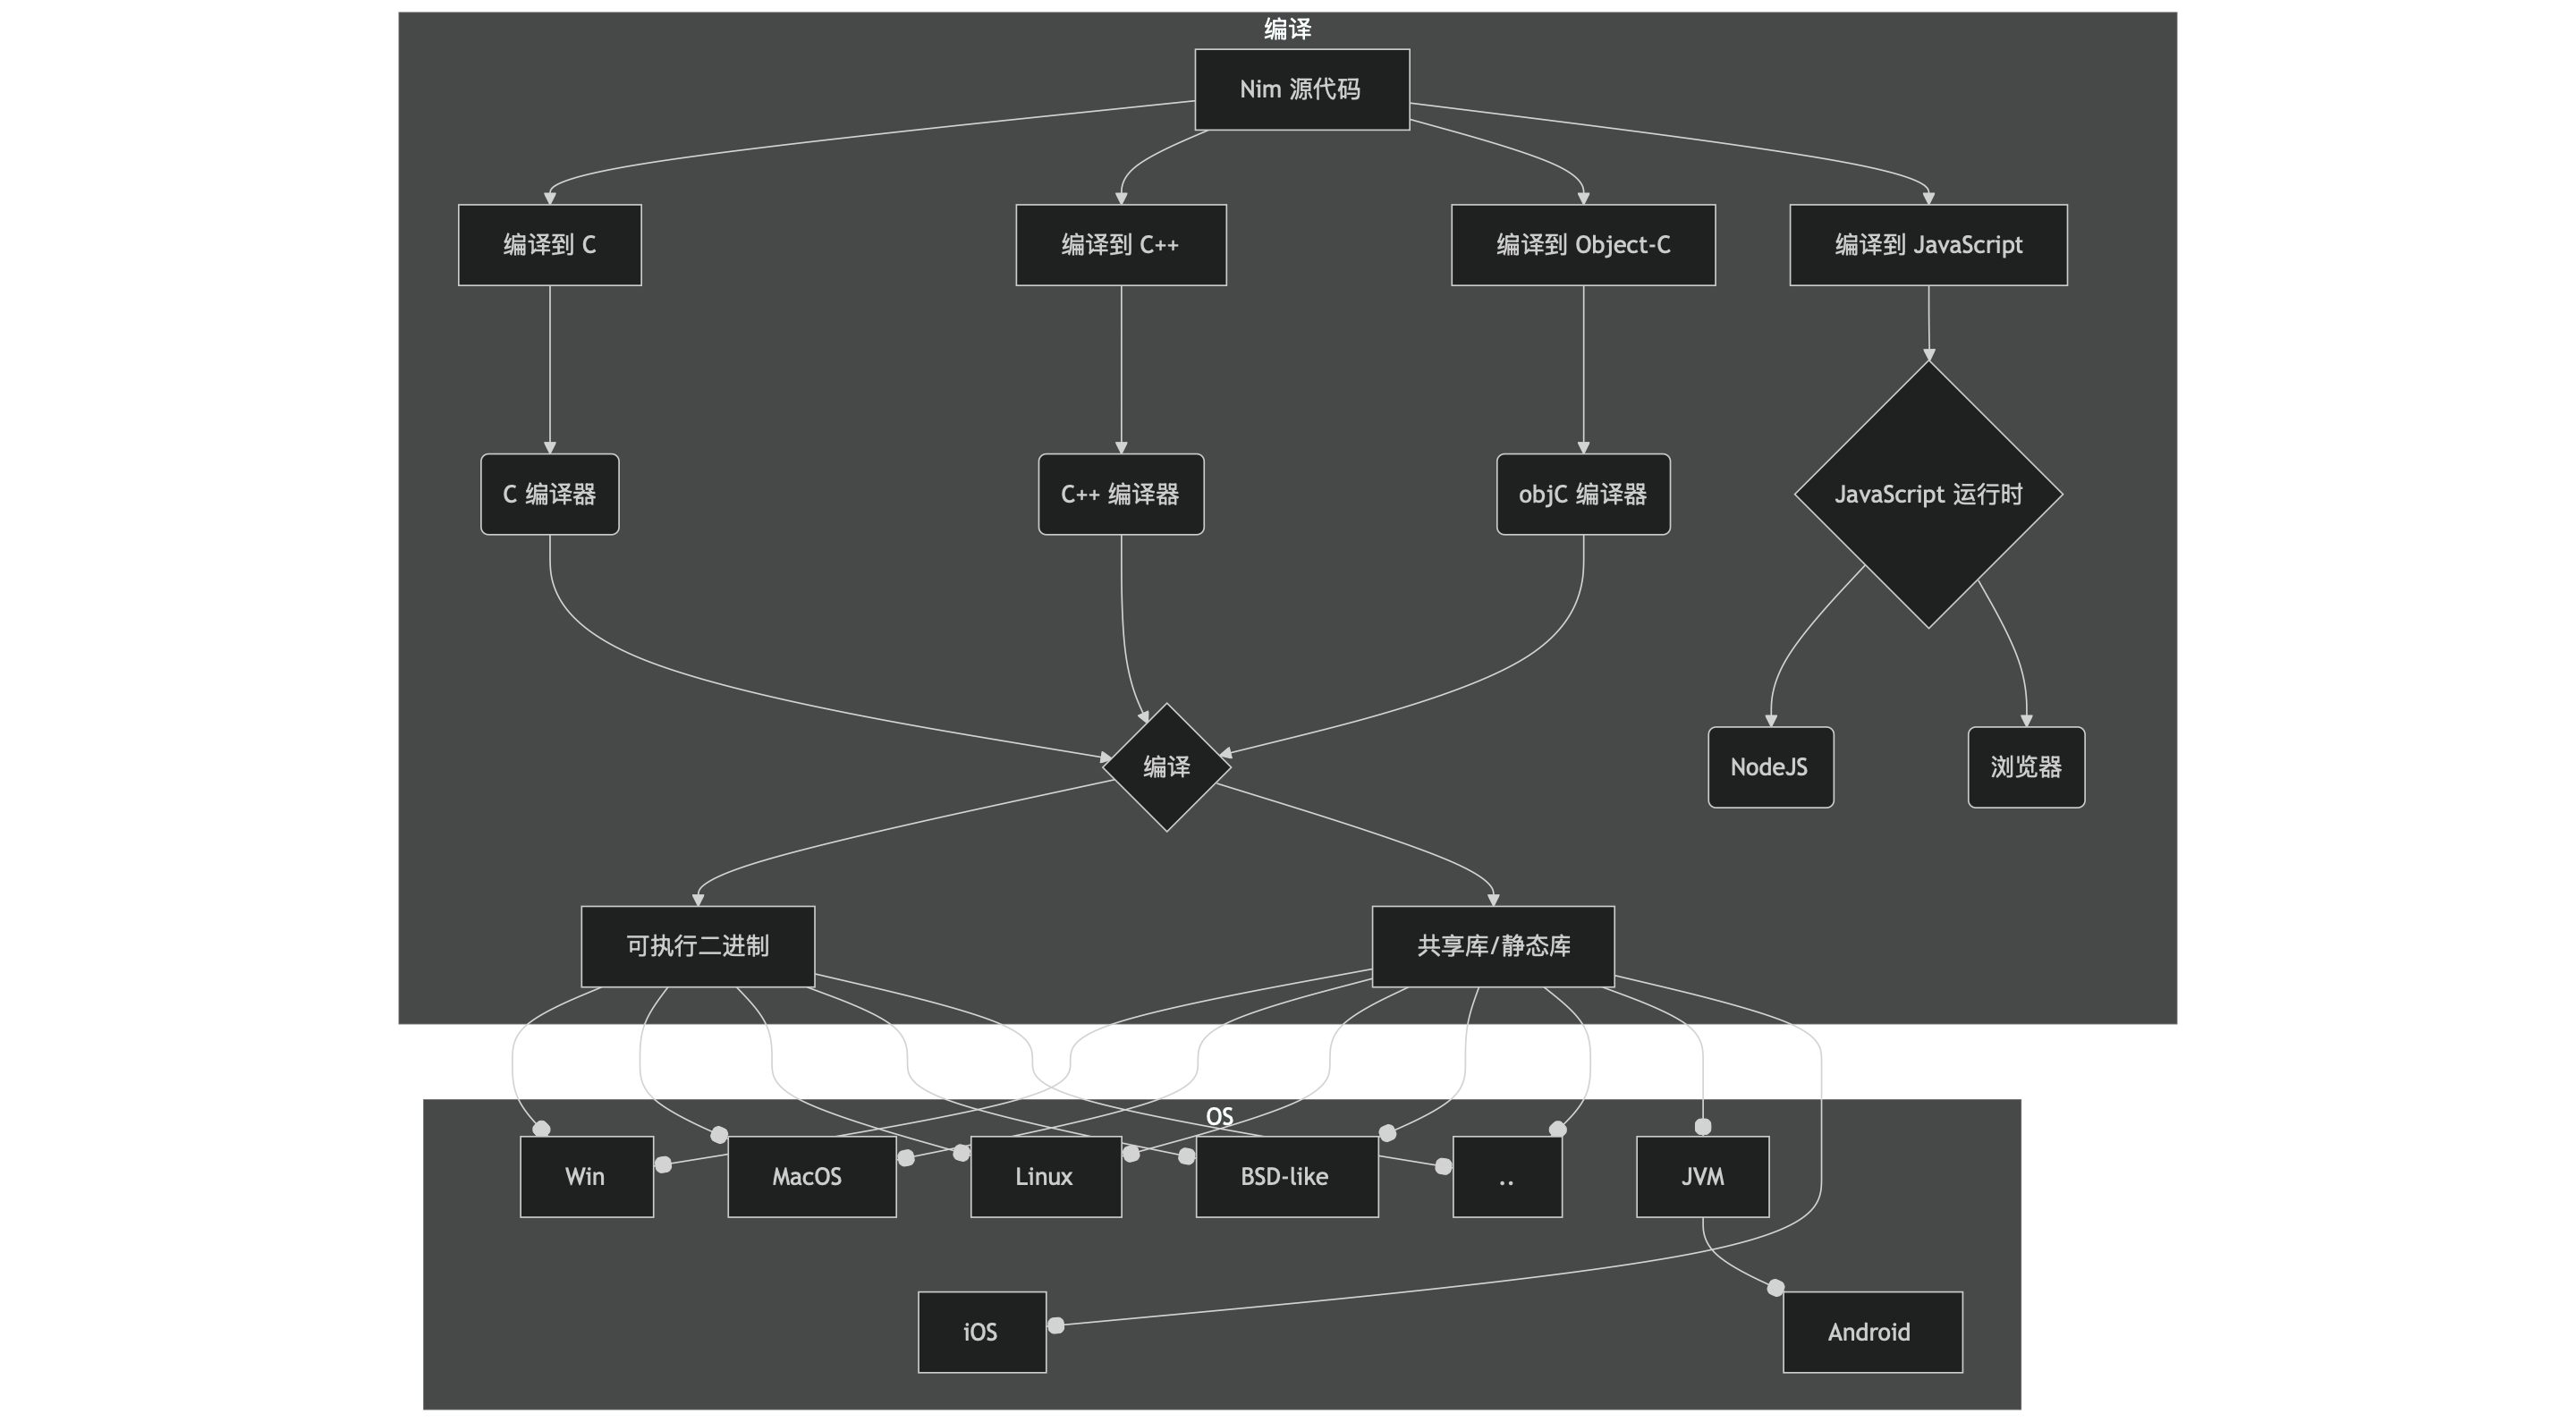
\includegraphics[width=\linewidth]{workflow_2.png}
		\caption{Workflow}
		\label{fig:workflow}
	\end{figure}
	\subsubsection{本机编译} %2.3.1
	\begin{itemize}[leftmargin=3.5em]
		\item 安装Nim编译器: \\
		\underline{\url{https://nim-lang.org/install.html}}
		\item 通过如下指令验证是否成功安装: 
		\begin{tcolorbox}[colback=gray!20, colframe=gray!20, rounded corners, boxrule=-5pt, height=0.01\textheight, width=0.18\textwidth, left=0pt, right=0pt, top=0pt, bottom=0pt]
			\begin{verbatim}
	nim --version
			\end{verbatim}
		\end{tcolorbox}
		\item 配置C编译器GCC / Clang
	\end{itemize}
	\subsubsection{交叉编译} %2.3.2
	\begin{itemize}[leftmargin=3.5em]
		\item 下载交叉编译工具链 \\
		LoongArch的开发需要编译工具链,具体步骤如下:
		\begin{enumerate}[leftmargin=1em]
				\item 通过如下网址找到适用于目标架构的工具链 \\
				\underline{\url{http://www.loongide.com/content/article.asp?style=nodate&typeid=26&id=150}}
				\item 选择对应工具链版本
		\end{enumerate}
		\item 配置Nim编译环境 \\
		Nim编译器需要进行配置以支持龙芯芯片架构,以下是基于LoongArch64所使用工具链演示:
		\begin{tcolorbox}[colback=gray!20, colframe=gray!20, rounded corners, boxrule=-5pt, height=0.08\textheight, width=0.9\textwidth, left=0pt, right=0pt, top=0pt, bottom=0pt]
			\begin{verbatim}
	export PATH=$PATH:/opt/toolchain-loongarch64-linux-gnu-gcc8-host-x86_64-
	2022-07-18/bin/
	export ARCH=loongarch64
	export CROSS_COMPILE=loongarch64-linux-gnu-
			\end{verbatim}
		\end{tcolorbox}
		之后输入如下命令进行编译(注:这是个例子,具体情况具体分析):
		\begin{tcolorbox}[colback=gray!20, colframe=gray!20, rounded corners, boxrule=-5pt, height=0.01\textheight, width=0.53\textwidth, left=0pt, right=0pt, top=0pt, bottom=0pt]
			\begin{verbatim}
	loongarch64-linux-gnu-gcc main.c -o main
			\end{verbatim}
		\end{tcolorbox}
	\end{itemize}
	\subsection{测试开发环境} %2.4
	为确保环境配置无误,运行以下测试程序:
	\begin{enumerate}[leftmargin=3.5em]
		\item 创建测试文件 \\
		创建一个简单的Nim程序hello.nim:
		\begin{tcolorbox}[colback=gray!20, colframe=gray!20, rounded corners, boxrule=-5pt, height=0.01\textheight, width=0.3\textwidth, left=0pt, right=0pt, top=0pt, bottom=0pt]
			\begin{verbatim}
	echo "Hello Loongson!"
			\end{verbatim}
		\end{tcolorbox}
		\item 编译并运行 \\
		使用交叉工具链编译:
		\begin{tcolorbox}[colback=gray!20, colframe=gray!20, rounded corners, boxrule=-5pt, height=0.03\textheight, width=0.58\textwidth, left=0pt, right=0pt, top=0pt, bottom=0pt]
			\begin{verbatim}
	wget http://example.com/toolchain.tar.gz
	tar -xzvf toolchain.tar.gz -C /opt/loongarch
			\end{verbatim}
		\end{tcolorbox}
		\item 验证生成的ELF文件 \\
		确认生成的二进制文件适用于Loongson架构:
		\begin{tcolorbox}[colback=gray!20, colframe=gray!20, rounded corners, boxrule=-5pt, height=0.01\textheight, width=0.14\textwidth, left=0pt, right=0pt, top=0pt, bottom=0pt]
			\begin{verbatim}
	file hello
			\end{verbatim}
		\end{tcolorbox}
		\item 运行 \\
		在龙芯机器上测试:
		\begin{tcolorbox}[colback=gray!20, colframe=gray!20, rounded corners, boxrule=-5pt, height=0.01\textheight, width=0.11\textwidth, left=0pt, right=0pt, top=0pt, bottom=0pt]
			\begin{verbatim}
	./hello
			\end{verbatim}
		\end{tcolorbox}
	\end{enumerate}
	\hspace*{2em}成功运行后,开发环境配置完成。

% 移植过程
\section{移植过程} %3
	\subsection{LoongArch平台的特性与挑战} %3.1
		\subsubsection{平台特性} %3.1.1
		\begin{itemize}[leftmargin=3.5em]
			\item 指令集架构:LoongArch是龙芯自主研发的指令集架构,具有32位和64位模式,支持丰富的矢量扩展指令。
			\item 独特寄存器集:包括通用寄存器(GPRs)、浮点寄存器(FPRs)、响亮寄存器(VEC)等,数量和布局与传统RISC架构不同。
			\item 内存管理:采用多级页表机制,支持打页、超大页和段式内存映射。
			\item 异常处理:异常向量表布局与传统MIPS架构存在类似,但偏移和一场代码分配有所不同。
		\end{itemize}
		\subsubsection{主要挑战} %3.1.2
		\begin{itemize}[leftmargin=3.5em]
			\item 指令兼容性:Nim编译器需要支持生成LoongArch特定的汇编指令。
			\item 启动代码适配:LoongArch的引导过程需要重新编写启动代码以支持新架构。
			\item 寄存器操作与调用约定:LoongArch使用独特的调用约定,需要在编译器后端中适配
		\end{itemize}
	\subsection{Nim编译器调整} %3.2
		\subsubsection{编译后端支持} %3.2.1
			\begin{enumerate}[leftmargin=3.5em]
				\item 修改Nim编译器的GCC后端配置文件(nim.cfg),添加对LoongArch平台的支持(仅交叉编译时必须):
				\begin{tcolorbox}[colback=gray!20, colframe=gray!20, rounded corners, boxrule=-5pt, height=0.08\textheight, width=0.54\textwidth, left=0pt, right=0pt, top=0pt, bottom=0pt]
					\begin{verbatim}
	when hostCPU == "loongarch64":
		const
			gcc.exe = "loongarch64-linux-gnu-gcc"
			linker.exe = "loongarch64-linux-gnu-ld"
					\end{verbatim}
				\end{tcolorbox}
				\item 为LoongArch平台启用特定的编译选项:
				\begin{tcolorbox}[colback=gray!20, colframe=gray!20, rounded corners, boxrule=-5pt, height=0.01\textheight, width=0.22\textwidth, left=0pt, right=0pt, top=0pt, bottom=0pt]
					\begin{verbatim}
	--cpu:loongarch64
					\end{verbatim}
				\end{tcolorbox}
			\end{enumerate}
		\subsubsection{适配调用约定} %3.2.2
			\begin{enumerate}[leftmargin=3.5em]
				\item 根据LoongArch的函数调用约定,调整参数传递规则:
				\begin{itemize}[leftmargin=1em]
					\item 前8个整形参数通过寄存器a0到a7传递,剩余参数通过堆栈传递。
					\item 返回值存放在a0 (或a0/a1)中。
				\end{itemize}
			\end{enumerate}
		\subsubsection{特定指令支持} %3.2.3
			\begin{enumerate}[leftmargin=3.5em]
				\item 如果需要直接生成特定LoongArch指令(如原子操作指令amadd.d),可使用Nim的\href{https://nim-lang.org/docs/manual.html#statements-and-expressions-assembler-statement}{\underline{内联汇编}}\\支持: \\ 注:以下的\$0, \$1, \$2实际书写时应替换为寄存器名,如a0、a1、a2等, 且Loongarch汇编中寄存器需用\$前缀。
				\begin{tcolorbox}[colback=gray!20, colframe=gray!20, rounded corners, boxrule=-5pt, height=0.05\textheight, width=0.23\textwidth, left=0pt, right=0pt, top=0pt, bottom=0pt]
					\begin{verbatim}
	asm """
	amadd.d $0, $1, $2
	"""
					\end{verbatim}
				\end{tcolorbox}
			\end{enumerate}
	\subsection{LoongArch64 CPU的启动} %3.3
		\subsubsection{启动流程概述} %3.3.1
		LoongArch启动代码流程与传统架构类似,主要包括以下步骤:
		\begin{enumerate}[leftmargin=3.5em]
			\item 初始化栈指针(sp)。
			\item 设置异常向量表。
			\item 初始化内存和页表。
			\item 跳转到内核主函数。
		\end{enumerate}
	\subsection{寄存器与内存布局设置} %3.4
		\subsubsection{寄存器初始化} %3.4.1
		\begin{enumerate}[leftmargin=3.5em]
			\item 全局寄存器配置
			\begin{enumerate}[leftmargin=1em]
				\item csr\_crmd: CPU当前模式寄存器,设置内核模式。
				\item csr\_asid: 地址空间标识寄存器,用于虚拟内存管理。
			\end{enumerate}
			\item 通用寄存器初始化
			在初始化阶段,清零所有通用寄存器,保留sp, gp等必要寄存器:
			\begin{tcolorbox}[colback=gray!20, colframe=gray!20, rounded corners, boxrule=-5pt, height=0.08\textheight, width=0.2\textwidth, left=0pt, right=0pt, top=0pt, bottom=0pt]
				\begin{verbatim}
	li t0, 0
	mv a0, t0
	mv a1, t0
	# 其他寄存器类似
				\end{verbatim}
			\end{tcolorbox}
		\end{enumerate}
		\subsubsection{内存布局设计} %3.4.2
		\begin{enumerate}[leftmargin=3.5em]
			在link.ld链接脚本中定义内存段:
			\begin{tcolorbox}[colback=gray!20, colframe=gray!20, rounded corners, boxrule=-5pt, height=0.24\textheight, width=0.23\textwidth, left=0em, right=0pt, top=0pt, bottom=0pt]
				\begin{verbatim}
	SECTIONS {
    	. = 0x80000000;
	.text : {
    *(.text) }
	.rodata : {
    *(.rodata) } 
	.data : {
    *(.data)} 
	.bss : {
    *(.bss) }
	}
				\end{verbatim}
			\end{tcolorbox}	
		\end{enumerate}
	\subsection{std/posix} %3.5
		\subsubsection{std/posix介绍} %3.5.1
		std/posix模块提供了与POSIX标准相关的功能,使得Nim程序能够在类Unix系统上进行低级操作,例如文件管理、进程控制和系统调用。\\ \hspace*{2em}这一模块对系统的调用进行封装,使得开发者可以使用Nim语言的语法进行系统级编程,增强了程序的可移植性。 \\ \hspace*{2em}具体内容见:\underline{\url{https://nim-lang.org/docs/posix.html}}
		\subsubsection{主要功能} %3.5.2
		\begin{enumerate}[leftmargin=3.5em]
    			\item 文件和目录操作:
     		\begin{itemize}[leftmargin=1em]
     			\item 提供了创建、删除、重命名和遍历目录的功能。
        			\item 支持文件权限的修改以及文件属性的查询。
    			\end{itemize}
   			\item 进程管理:
    			\begin{itemize}[leftmargin=1em]
        			\item 可以创建子进程,并支持进程的同步和通信。
        			\item 提供了对进程状态的监控功能。
    			\end{itemize}
    			\item 信号处理:
    			\begin{itemize}[leftmargin=1em]
    				\item 提供了设置和捕获POSIX信号的能力,使程序能够对异步事件作出反应。
    			\end{itemize}
    			\item 线程支持:
    			\begin{itemize}[leftmargin=1em]
        			\item 提供了多线程编程的接口,允许创建和管理线程。
        			\item 支持互斥锁和条件变量,以确保线程安全。
    			\end{itemize}
		\end{enumerate}
		\subsubsection{移植注意事项} %3.5.3
		\begin{enumerate}[leftmargin=3.5em]
    			\item 系统调用的兼容性:确保所有使用的POSIX系统调用在LoongArch架构上都能正确执行,特别是涉及底层操作的函数。
			\item 编译器支持:检查LoongArch的编译器是否支持Nim的特性,尤其是与POSIX相关的扩展。
   		 	\item 性能优化:评估在LoongArch上执行的性能,可能需要进行特定的优化,以确保与其他架构的兼容性和性能一致性。
    			\item 测试用例:编写对std/posix功能的单元测试,确保在LoongArch架构上正确运行,并与预期结果一致。
		\end{enumerate}

% 错误信息筛选与处理(Main_01)
\section{错误信息筛选与处理} %4
	进行Nim的测试过程中,./koch test 默认在工作目录(即./testresults)下生成测试结果文件,结构为:
	\begin{center}
	\begin{tcolorbox}[colback=gray!20, colframe=gray!20, rounded corners, boxrule=-5pt, height=0.06\textheight, width=0.62\textwidth, left=0pt, right=0pt, top=0pt, bottom=0pt]
		\begin{verbatim}
		category/testName.json
		category为测试类型,如“compiler”、“tools”等,
		testName为测试名称,如“t001”、“t002”等。
		\end{verbatim}
	\end{tcolorbox}
	\end{center}
	\subsection{测试结果解析与管理} %4.1
	这个过程是遍历并指定目录及其子目录下的所有JSON文件,逐文件解析内容,过滤出未成功的记录并对记录进行筛选(删除重复字段)和结构化(转换字段类型),最后将非空数据以FileRecord的形式返回。得到的json文件见\href{run:../testresult/}{$ \sim/nim\_testresult/ $} % TODO: 加入文件超链接以便快速查询
	\begin{enumerate}[leftmargin=3.5em]
		\item 定义RunRecord和FileRecord类型,存储与测试相关的数据,包括测试状态、后段类型、命令行参数等。
		\begin{tcolorbox}[colback=gray!20, colframe=gray!20, rounded corners, boxrule=-5pt, width=0.74\textwidth, left=0pt, right=0pt, top=0pt, bottom=0pt]
			\begin{verbatim}
	# RunRecord
	iterator filterNonSuccess*(arrNode: JsonNode): RunRecord =
		for node in arrNode:
			if "reSuccess" == node["result"].getStr():
				continue
						
			let target = node["target"].getStr()
			for field in DupFields:
				node.delete field
						
			var argvJoined = node["name"].getStr
			var argv = argvJoined.split ' '
			node["name"] = newJString argv[0]
			argv.delete 0
			var res: RunRecord
					
			res.status = node.popEnumKey[:TResultEnum]("result")
			res.backend = node.popEnumKey[:Backend]("target")
					
			res.node = node
			res.args = argv
			yield res
					
	# FileRecord
	using dir: string proc parseFile*(dir; filename: string):
	Option[FileRecord] =
			## returns none iff file is empty
			let path = dir/filename
			var fstr: FileStream
			if not fstr.openMayAfterFixJson path:
				return
			assert not fstr.isNil
			defer: fstr.close
			var res: FileRecord
			res.name = filename
			res.name.removeSuffix".json"
			for i in fstr.filterNonSuccess filename:
				res.data.add i
			result = some res
			\end{verbatim}
		\end{tcolorbox}
		\item 使用JSON数据结构来表示测试结果,通过解析和处理JSON文件,实现对测试状态的分析。
	\end{enumerate}
	\subsection{状态管理} %4.2
	\begin{enumerate}[leftmargin=3.5em]
		\item 定义getAllStatus()函数用于手机所有测试记录中出现的状态,利用集合(HashSet)来避免重复。
		\begin{tcolorbox}[colback=gray!20, colframe=gray!20, rounded corners, boxrule=-5pt,height=0.08\textheight , width=0.54\textwidth, left=0pt, right=0pt, top=0pt, bottom=0pt]
			\begin{verbatim}
	# getAllStatus()
	proc getAllStatus*: HashSet[TResultEnum] =
		template doWith(d) = result.incl d.status
		dir.doWithNonSuccNode doWith
			\end{verbatim}
		\end{tcolorbox}
		\item 定义getStatusDiffMap()函数通过状态分类,将测试记录分组存储在表(Table)中,便于后续查看和分析。
		\begin{tcolorbox}[colback=gray!20, colframe=gray!20, rounded corners, boxrule=-5pt, height=0.18\textheight, width=0.76\textwidth, left=0pt, right=0pt, top=0pt, bottom=0pt]
			\begin{verbatim}
	# getStatusDiffMap()
	proc getStatusDiffMap*: Table[TResultEnum, seq[RunRecord]] =
	# result = initTable[TResultEnum, seq[RunRecord]]()
	template doWith(d) =
		if d.status not_in result:
			result[d.status] = @[]
		result[d.status].add d
	dir.doWithNonSuccNode doWith
			\end{verbatim}
		\end{tcolorbox}
	\end{enumerate}
	\subsection{文件处理与修复} %4.3
	这个过程是修复和打开可能存在格式问题的JSON文件,并将其内容加载为文件流。
	\begin{enumerate}[leftmargin=3.5em]
		\item 定义openMayAfterFixJson()函数在打开文件时检查并修复文件格式,确保数据能够正确解析。
		\item 其中包括读取并处理JSON文件,包括自动修复可能缺失的JSON结构(如缺少闭合的 ‘]’)。
		\begin{tcolorbox}[colback=gray!20, colframe=gray!20, rounded corners, boxrule=-5pt, height=0.2\textheight, width=0.45\textwidth, left=0pt, right=0pt, top=0pt, bottom=0pt]
			\begin{verbatim}
	let arrEnded = f.readChar() == ']'
				
	if arrStarted and not arrEnded:
		f.truncate()
		f.write ']'
		f.flushFile()
					
	f.setFilePos(0, fspSet)
	result = true
			\end{verbatim}
		\end{tcolorbox}
	\end{enumerate}
	\subsection{输出与格式化} %4.4
	这个过程是将测试运行得到的数据进行格式化为Markdown列表。\\ 具体内容见\href{run:../loongson_testresult.md}{$ \sim/nim\_testresult/loongson\_testresult.md $} % TODO: 加入文件超链接以便快速查询
	\begin{enumerate}[leftmargin=3.5em]
		\item 利用MarkdownList类型,生成Markdown格式的输出,便于在测试结果生成后以结构化的形式展示测试结果。
		\begin{tcolorbox}[colback=gray!20, colframe=gray!20, rounded corners, boxrule=-5pt, height=0.2\textheight, width=0.83\textwidth, left=0pt, right=0pt, top=0pt, bottom=0pt]
			\begin{verbatim}
	using self: MarkdownList
	func `\$`*(self; nSpace=self.nSpace; appendNewLine=true): string =
 	let spaces = ' '.repeat nSpace
  		for line in self.lines:
    			result.add spaces
    			result.add self.prefix
    			result.add line
    			result.add '\n'
  		if appendNewLine: result.add '\n'
			\end{verbatim}
		\end{tcolorbox}
		\item 提供asCode()和toInlineCode()方法来处理输出格式,增强可读性和信息传递。
		\begin{tcolorbox}[colback=gray!20, colframe=gray!20, rounded corners, boxrule=-5pt, height=0.25\textheight, width=0.7\textwidth, left=0pt, right=0pt, top=0pt, bottom=0pt]
			\begin{verbatim}
	# asCode()
	func asCode(s: var string; lang=""; default="*None*") =
  	if s.len == 0:
    		s = default
    		return
  	s = '\n' & "```"& lang & '\n' & s
  	if s[^1] not_in {'\n', '\r'}: s.add '\n'
  	s = indent(s & "```", IndentSpaceN)
			
	# toInlineCode()
	func toInlineCode(s: string): string = '`' & s & '`'
			\end{verbatim}
		\end{tcolorbox}
	\end{enumerate}
	\subsection{主程序逻辑} %4.5
	\begin{enumerate}[leftmargin=3.5em]
		\item 使用$ when\:isMainModule $结构来确保只有在直接运行该文件时才执行相关逻辑,这样可以方便地将代码作为模块导入而不执行主逻辑。
		\item 调用getAllStatus()和echoStatusDiffMap()函数以打印出测试状态和状态对应的详细信息。
		\begin{tcolorbox}[colback=gray!20, colframe=gray!20, rounded corners, boxrule=-5pt, height=0.11\textheight, width=0.4\textwidth, left=0pt, right=0pt, top=0pt, bottom=0pt]
			\begin{verbatim}
	import parseTestamentJson/mains

	when isMainModule:
  		echo getAllStatus()
  		echoStatusDiffMap()
			\end{verbatim}
		\end{tcolorbox}
	\end{enumerate}
	\hspace*{2em}(详细内容见:{\underline{\url{https://github.com/nimigrate/parseTestamentJson.git}}})

% 代码实现(Main_02)
\section{代码实现} %5
	\subsection{问题解决} %5.1
		\subsubsection{高级语言迁移} %5.1.1
		涉及修正内容过多,这里举几个例子,其他修改请见$ \sim/build\_nim/gitlab-eduxiji-repo/src $ % TODO: 链接到仓库对应目录
		\begin{itemize}[leftmargin=3.5em]
			\item 进行对$ socketstreams.nim $和$ thttpclient\_ssl.nim $测试时,如果采用$ --cpu:mips64el $架构编译会失败。具体代码如下所示:
			\begin{tcolorbox}[colback=gray!20, colframe=gray!20, rounded corners, boxrule=-5pt, width=0.8\textwidth, left=0pt, right=0pt, top=0pt, bottom=0pt]
				\begin{verbatim}
	discard """
	matrix: "--mm:refc; --mm:orc"
  	output: '''
	OM
	NIM
	3
	NIM
	NIM
	Hello server!
	Hi there client!
	'''"""
	import std/socketstreams, net, streams

	block UDP:
  		var recvSocket = newSocket(AF_INET, SOCK_DGRAM, IPPROTO_UDP)
  		var recvStream = newReadSocketStream(recvSocket)
  		recvSocket.bindAddr(Port(12345), "127.0.0.1")

  		var sendSocket = newSocket(AF_INET, SOCK_DGRAM, IPPROTO_UDP)
  		sendSocket.connect("127.0.0.1", Port(12345))
  		var sendStream = newWriteSocketStream(sendSocket)
  		sendStream.write "NOM\n"
  		sendStream.setPosition(1)
  		echo sendStream.peekStr(2)
  		sendStream.write "I"
  		sendStream.setPosition(0)
  		echo sendStream.readStr(3)
  		echo sendStream.getPosition()
  		sendStream.flush()

  		echo recvStream.readLine()
 	 	recvStream.setPosition(0)
  		echo recvStream.readLine()
  		recvStream.close()

	block TCP:
  		var server = newSocket()
  		server.setSockOpt(OptReusePort, true)
  		server.bindAddr(Port(12345))
  		server.listen()
				\end{verbatim}
			\end{tcolorbox}
			\newpage
			\begin{tcolorbox}[colback=gray!20, colframe=gray!20, rounded corners, boxrule=-5pt, width=0.8\textwidth, left=0pt, right=0pt, top=0pt, bottom=0pt]
				\begin{verbatim}
	var
    		client = newSocket()
    		clientRequestStream = newWriteSocketStream(client)
    		clientResponseStream = newReadSocketStream(client)
  	client.connect("127.0.0.1", Port(12345))
  	clientRequestStream.writeLine("Hello server!")
  	clientRequestStream.flush()
			
  	var
    		incoming: Socket
    		address: string
  	server.acceptAddr(incoming, address)
  	var
    		serverRequestStream = newReadSocketStream(incoming)
    		serverResponseStream = newWriteSocketStream(incoming)
  	echo serverRequestStream.readLine()
  	serverResponseStream.writeLine("Hi there client!")
  	serverResponseStream.flush()
  	serverResponseStream.close()
  	serverRequestStream.close()

  	echo clientResponseStream.readLine()
  	clientResponseStream.close()
	clientRequestStream.close()
				\end{verbatim}
			\end{tcolorbox}
			分析: \\
			\hspace*{2em}MIPS和LoongArch64架构在实现网络相关的系统调用时,会有不同的约定和支持的功能。包括套接字选项SO\_REUSEPORT的实现和可用性。在MIPS架构上,SO\_REUSE-\\PORT的值为0x0200,而在LoongArch64架构上,其值为15,可知该选项在MIPS中和在LoongArch上得到的结果不同。 \\
			\hspace*{2em}考虑到第一版Nim编译器时将Nim代码编译成C代码,而C代码本身在处理不同的套接字选项时可能未能考虑到不同架构的实现差异。特别是如果在编译时未能正确检测到目标平台的特性,可能导致生成的代码出现问题。再者,C代码中的某些特性(如SO\_REUSEPORT的使用)可能在不同架构上没有经过充分测试,导致不兼容的情况。
		\end{itemize}
		\subsubsection{汇编语言迁移} %5.1.2
		LoongsonArch架构的汇编指令集在某些方面与intel格式相似,例如:
			\begin{itemize}[leftmargin=3.5em]
				\item 立即数无前缀:在龙芯汇编中,立即数(即直接给出的数值)通常不需要前缀。这意味着在指令中直接写出数值即可,不需要额外的符号来指明这是一个立即数。
   				\item reg(at\&t: \%):龙芯汇编中寄存器通常用 \$ 符号表示,这与 AT\&T 汇编语法中的 \% 符号相似。例如 \$r0 表示通用寄存器0,这种表示方法有助于区分寄存器和内存地址或立即数。
    				\item do dst, src:这是龙芯指令的格式,其中$ do $表示某种操作,$ dst  $是目标操作数(通常是寄存器或内存地址),而$ src $是源操作数。这种格式与Intel汇编中的$ instruction\:dst,\,src $类似,表示将源操作数$ src $进行某种操作后存储到目标操作数$ dst $中。
    				\item do.类型后缀:这是龙芯指令后缀,用于指定操作数的类型或大小。类似于intel\_x86架构中,$ add \:dword \:ptr[eax],\,ebx $中的$ dword\:ptr $指定了操作数的类型为32位。
			\end{itemize}
		\begin{itemize}[leftmargin=3.5em]
			\item 进行对$ tasm.nim $测试时发现龙芯不支持$ mov $指令。具体代码如下所示:
			\begin{tcolorbox}[colback=gray!20, colframe=gray!20, rounded corners, boxrule=-5pt, height=0.32\textheight, width=0.75\textwidth, left=0pt, right=0pt, top=0pt, bottom=0pt]
				\begin{verbatim}
	proc testAsm() = 
		let src = 41
		var dst = 0
		
		asm """
			mov %1, %0\n\t
			add $1, %0
			: "=r" (`dst`)
			: "r" (`src`)"""
		
		doAssert dst == 42
	when defined(gcc) or defined(clang) and not defined(cpp):
		{.passc: "-std=c99".}
		testAsm()
				\end{verbatim}
			\end{tcolorbox}
			运行结果如下:
			\begin{figure}[htbp]
				\centering
				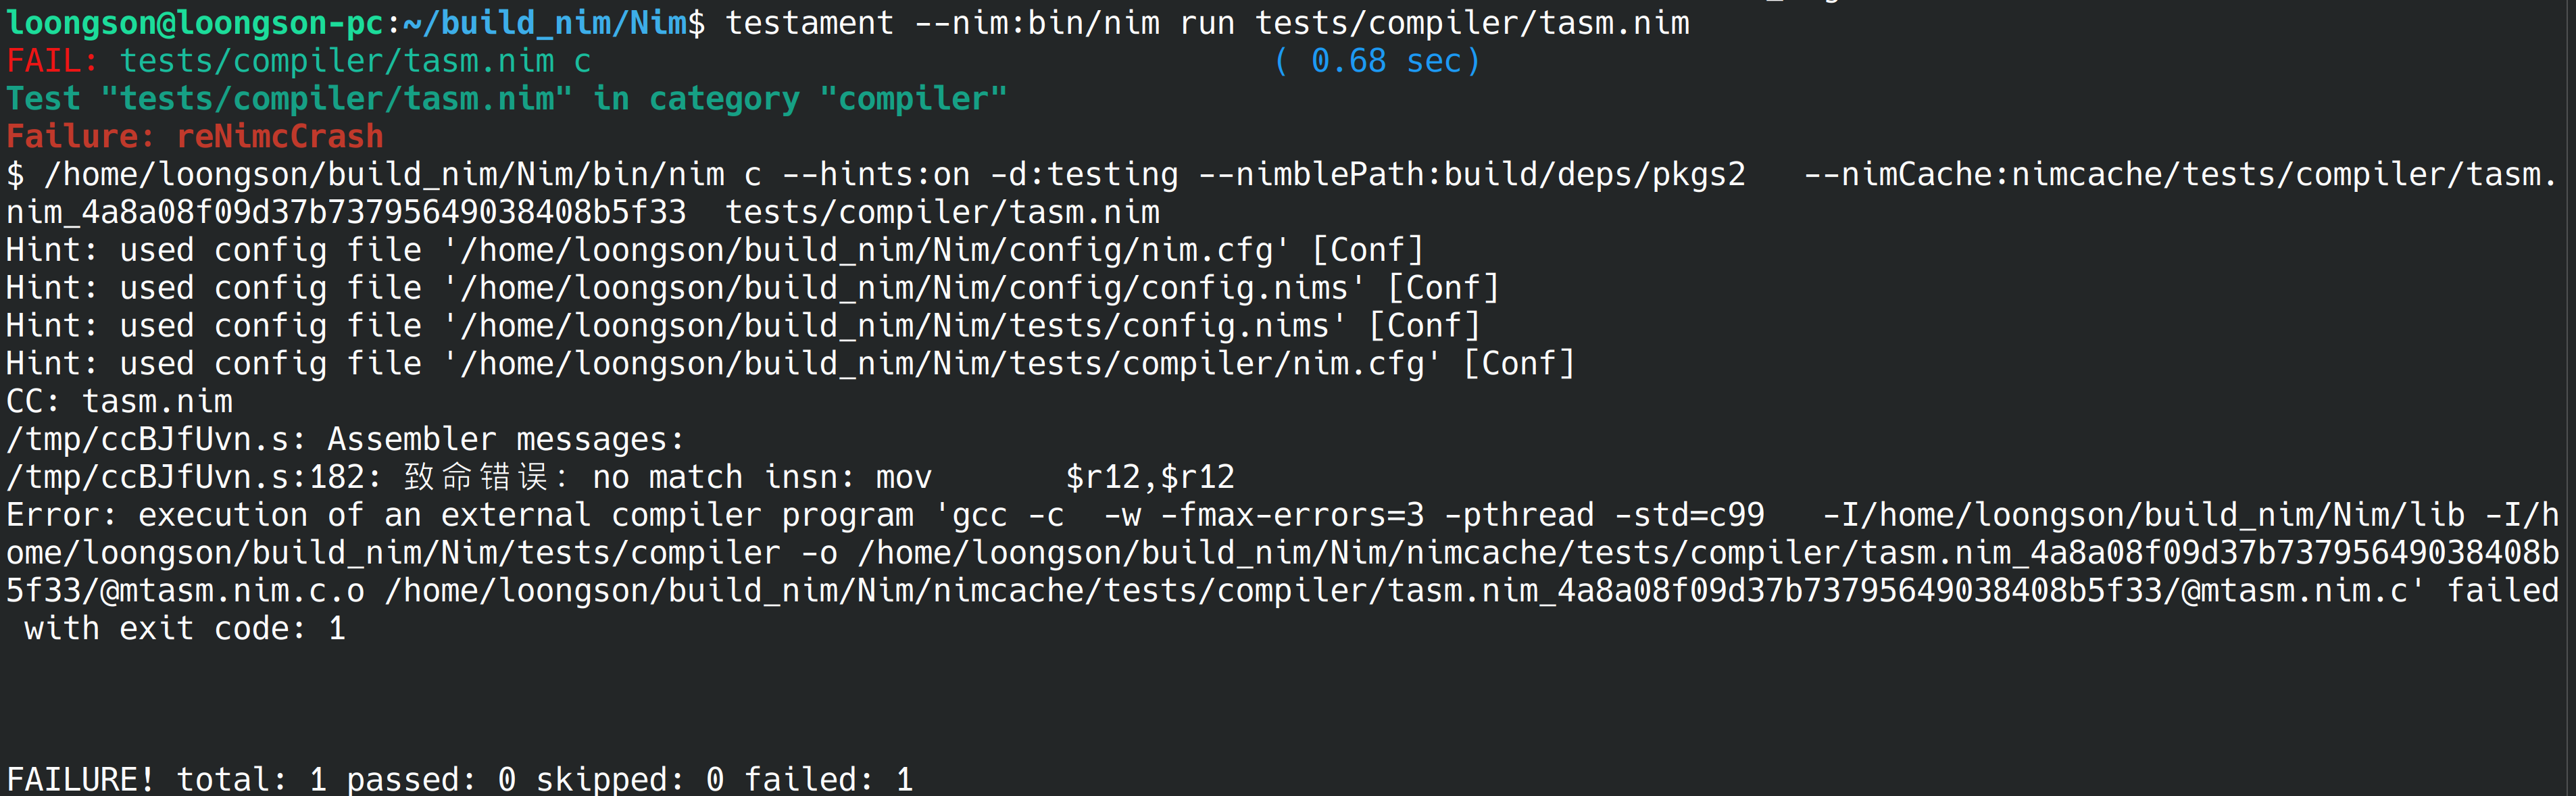
\includegraphics[width=\linewidth]{tasm_err_snap.png}
				\caption{tasm}
				\label{fig:tasm_err}
			\end{figure} \\
			分析:这其中的$ mov\:\$r12,\,\$12 $没有匹配,这是因为Loongson缺少$ mov $指令导致。 \\
			解决方案:
			\begin{tcolorbox}[colback=gray!20, colframe=gray!20, rounded corners, boxrule=-5pt, height=0.07\textheight, width=0.2\textwidth, left=0pt, right=0pt, top=0pt, bottom=0pt]
				\begin{verbatim}
	```asm
		mov %1, %0\n\t
		add $1, %0
	```
				\end{verbatim}
			\end{tcolorbox}
			将这部分代码修改为
			\begin{tcolorbox}[colback=gray!20, colframe=gray!20, rounded corners, boxrule=-5pt, height=0.01\textheight, width=0.23\textwidth, left=0pt, right=0pt, top=0pt, bottom=0pt]
				\begin{verbatim}
	`addi.w %0, %1, 1`
				\end{verbatim}
			\end{tcolorbox}
		\end{itemize}
	\subsection{其他问题} %5.2
		\subsubsection{LoongArch内置Node版本问题}  %5.2.1
		\begin{itemize}[leftmargin=3.5em]
			\item 在测试$ tnativeexc.nim $时,发现对于同一报错,每次报错信息都不一样,具体代码如下所示:
			\begin{tcolorbox}[colback=gray!20, colframe=gray!20, rounded corners, boxrule=-5pt, height=0.72\textheight, width=0.9\textwidth, left=0pt, right=0pt, top=0pt, bottom=0pt]
				\begin{verbatim}
	discard """
		action: "run"
	"""
	
	import jiffy
	
	# Can catch JS exceptions
	try:
  		asm """throw new Error('a new error');"""
	except JsError as e:
  		doAssert e.message == "a new error"
	except:
  		doAssert false

	# Can distinguish different exceptions
	try:
  		asm """JSON.parse(';;');"""
	except JsEvalError:
  		doAssert false
	except JsSyntaxError as se:
  		doAssert se.message == "Unexpected token ';', \";;\" is not valid JSON"
	except JsError as e:
  		doAssert false

	# Can catch parent exception
	try:
  		asm """throw new SyntaxError();"""
	except JsError as e:
  		discard
	except:
  		doAssert false
				\end{verbatim}
			\end{tcolorbox}
			运行结果如下:
			\newpage
			\begin{figure}[htbp]
				\centering
				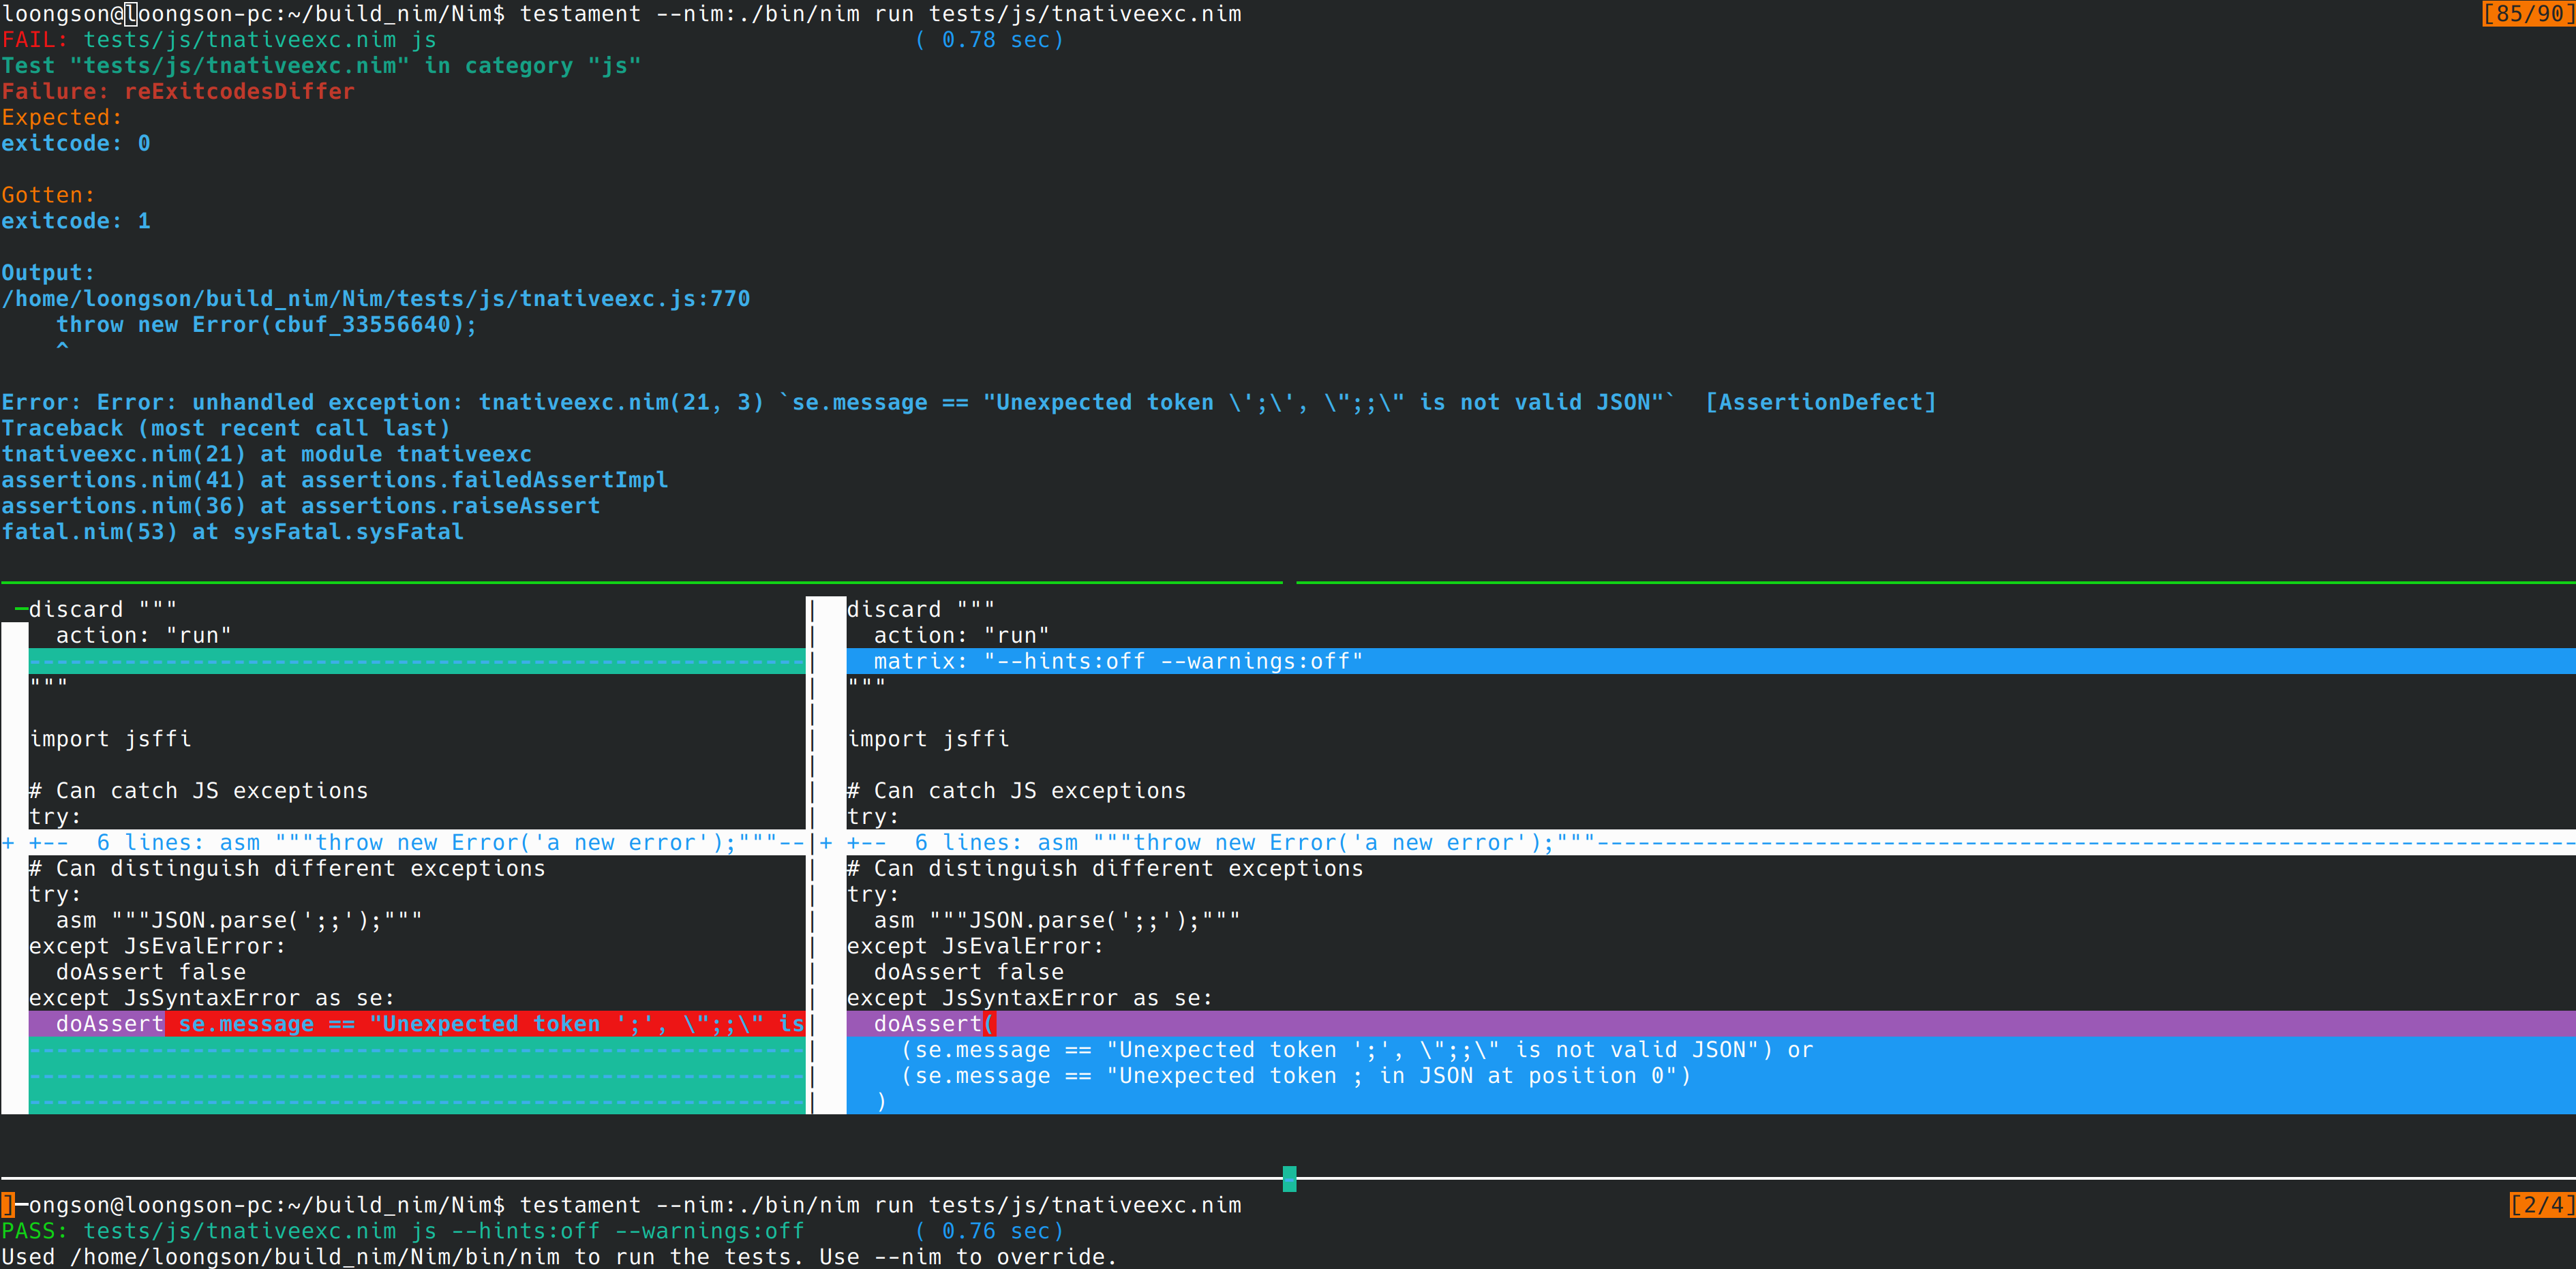
\includegraphics[width=\linewidth]{tnativeexc_fix_show.png}
				\caption{TasmDebug}
				\label{fig:node_err}
			\end{figure} \\
			分析:由此发现是因为环境导致的问题,即当前所使用Node版本过低,所以对于同一报错会有不同报错信息,从而导致测试失败。检查结果如下:
			\begin{figure}[htbp]
				\centering
				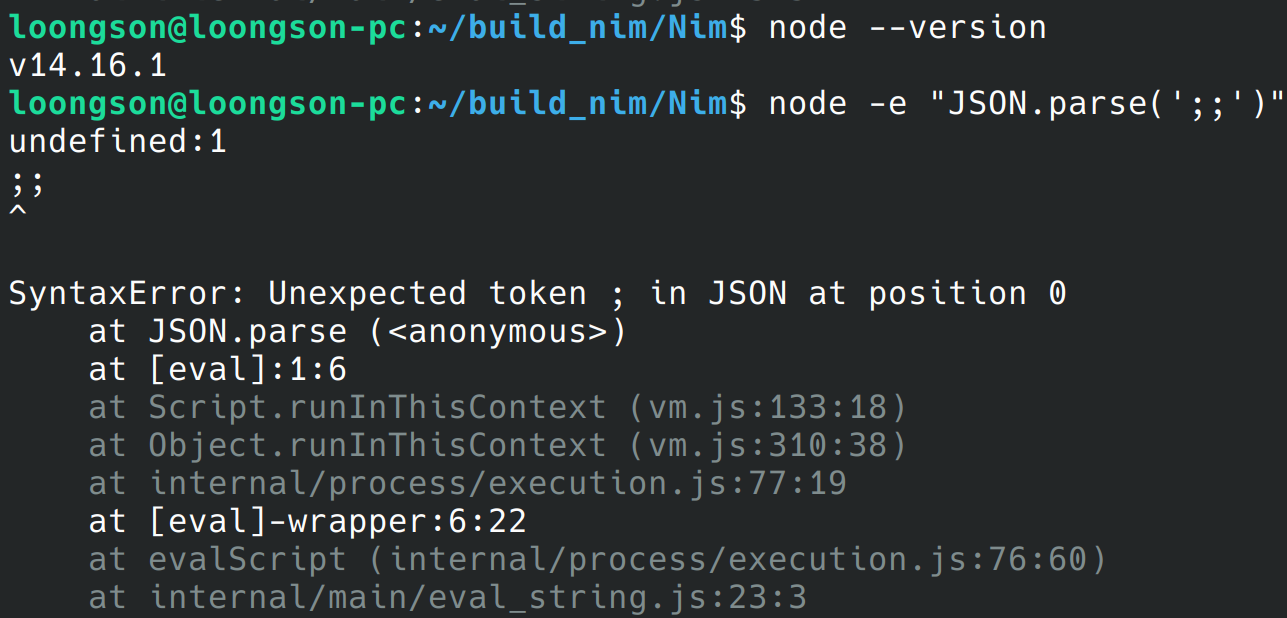
\includegraphics[width=0.8\linewidth]{tnativeexc_node_err_msg.png}
				\caption{Node}
				\label{fig:tasm_err}
			\end{figure}
		\end{itemize}
		\subsubsection{命令行参数问题} %5.2.2
		\begin{itemize}[leftmargin=3.5em]
			\item Nim有一个命令行参数$ --asm $,用于生成asm代码,当在LoongArch下执行时,编译器会报错:
			\begin{tcolorbox}[colback=gray!20, colframe=gray!20, rounded corners, boxrule=-5pt, height=0.01\textheight, width=0.73\textwidth, left=0pt, right=0pt, top=0pt, bottom=0pt]
				\begin{verbatim}
	gcc: error: unrecognized command line option ‘-masm=intel’
				\end{verbatim}
			\end{tcolorbox}
			检查后发现,Nim源码的$ extccomp.nim $有
			\begin{tcolorbox}[colback=gray!20, colframe=gray!20, rounded corners, boxrule=-5pt, height=0.01\textheight, width=0.8\textwidth, left=0pt, right=0pt, top=0pt, bottom=0pt]
				\begin{verbatim}
	gnuAsmListing = "-Wa,-acdl=$asmfile -g -fverbose-asm -masm=intel"
				\end{verbatim}
			\end{tcolorbox}
			而LoongArch的汇编既不是AT\&T格式,也不是intel格式,而是MIPS系,所以不接受$ -masm=intel $参数(即$ -masm $用于切换生成汇编格式是intel格式还是AT\&T格式)。
			之后发现$ -Wa $,表示给汇编器传参,具体如下: \\
			\begin{tcolorbox}[colback=gray!20, colframe=gray!20, rounded corners, boxrule=-5pt, height=0.01\textheight, width=0.24\textwidth, left=0pt, right=0pt, top=0pt, bottom=0pt]
				\begin{verbatim}
	-Wa, acdl=$asmfile
				\end{verbatim}
			\end{tcolorbox}
			不会导致LoongArch的GCC生成名为 \$asmfile的汇编代码文件。因此这个问题需要之后向GCC提交issue。
			考虑到的解决方案有:增添$ -S $参数,这样能使GCC生成汇编代码,但是会造成生成文件后缀名为$ .s $,而Nim期望生成文件后缀为$ .asm $。参考文档详见:\underline{\url{https://nim-lang.org/docs/nimc.html}}
		\end{itemize}
		\subsubsection{文档格式修复} %5.2.3
		\begin{enumerate}[leftmargin=3.5em]
			\item 在查阅文档时偶然间发现了"loongarch64"错误,具体如下:
			\begin{figure}[htbp]
				\centering
				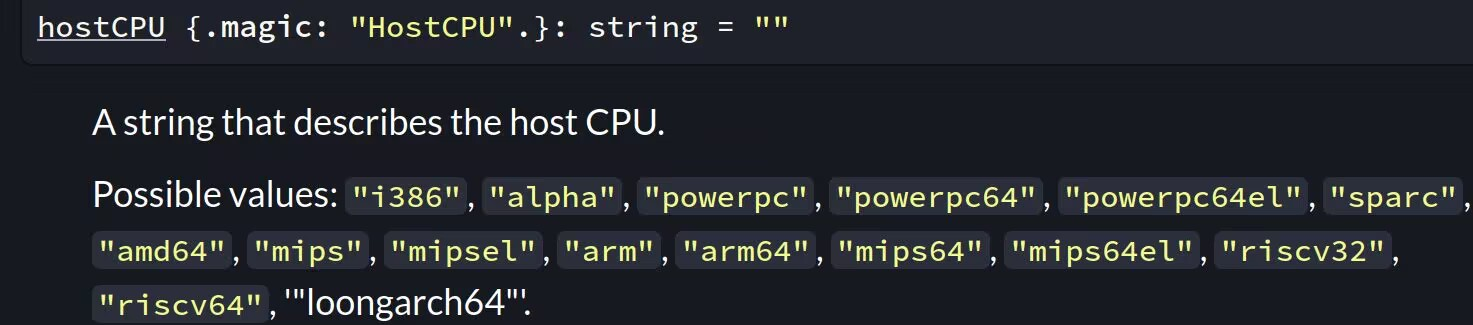
\includegraphics[width=0.8\linewidth]{loongarch64Format.png}
				\caption{Format}
				\label{fig:format_err}
			\end{figure} \\
			经过上报官方Nim,确认这是一个文档格式的修复。详见: \\
			\underline{\url{https://github.com/nim-lang/Nim/pull/23621}}
		\end{enumerate}

% 性能优化与问题解决
\section{性能优化与问题解决} %6
	\subsection{编译优化策略} %6.1
	\begin{enumerate}[leftmargin=3.5em]
		\item 启用LoongArch特定优化选项,如矢量化和流水线优化。
		\item 利用Nim的内嵌C代码功能,直接调用高校的底层库函数。
	\end{enumerate}
	\subsection{常见问题与解决方法} %6.2
	\begin{enumerate}[leftmargin=3.5em]
		\item 问题1:工具链配置错误 \\ 解决方案:检查PATH和交叉编译工具链是否正确配置。
		\item 问题2:系统调用失败 \\ 解决方案:验证POSIX接口的实现是否与LoongArch平台兼容。
	\end{enumerate}

% 未来计划与改进方向
\section{预期效果与未来计划} %7
	\subsection{预期效果} %7.1
	\begin{enumerate}[leftmargin=3.5em]
		\item 完善国产龙芯芯片的生态
		\item 为软件国产化提供更优方案进行探索
		\item 完成Nim语言编译器在国产龙芯芯片下的迁移,提高Nim的跨平台性
		\item 推进Nim在软件开发中的应用
	\end{enumerate}
	\subsection{未来计划} %7.2
	\begin{enumerate}[leftmargin=3.5em]
		\item 增加对更多LoongArch特性的支持
		\item 测试LoongArch新版本ABI的支持
		\item 优化Nim编译器生成代码的性能,使其更适合龙芯平台
		\item 扩展第三方库的功能,以支持更多的LoongArch应用场景
	\end{enumerate}

% 附录
\section{附录} %8
	\subsection{项目相关工具使用指南} %8.1
	\begin{enumerate}[leftmargin=3.5em]
		\item 交叉编译工具链下载和安装:
		\begin{itemize}[leftmargin=1em]
			\item 从\underline{\url{https://www.loongide.com}}获取最新版工具链。
			\item 配置环境变量以使用工具链。
		\end{itemize}
		\item 调试工具使用:% TODO: 加入什么,问lim
		\begin{itemize}[leftmargin=1em]
			\item GDB(GNU Debugger)
			\item GCC(GNU Compiler Collection)
		\end{itemize}
	\end{enumerate}
	\subsection{参考资料} %8.2
	\begin{itemize}[leftmargin=3.5em]
		\item Nim官方文档 \underline{\url{https://nim-lang.org/documentation.html}}
		\item 龙芯中科官网 \underline{\url{https://www.loongson.cn/system/loongarch}}
		\item Nim官方GitHub仓库 \underline{\url{https://github.com/nim-lang/Nim}}
		\item Nim支持LoongArch架构官方文档 \underline{\url{https://nim-lang.org/docs/system.html\#hostCPU}}
	\end{itemize}

\end{document}
